\documentclass[11pt,a4paper]{article}

\usepackage[margin=2.5cm]{geometry}
\usepackage[T1]{fontenc}
\usepackage{lmodern}
\usepackage{microtype}
\usepackage{amsmath,amssymb,amsthm}
\usepackage{graphicx}
\usepackage{booktabs}
\usepackage{multirow}
\usepackage{xcolor}
\usepackage{tikz}
\usetikzlibrary{positioning,arrows.meta,fit}
\usepackage{caption}
\usepackage[section]{placeins}
\usepackage[hidelinks]{hyperref}
\usepackage{cleveref}

\graphicspath{{../figures/}}
\captionsetup{font=small,labelfont=bf}
\newtheorem{proposition}{Proposition}
\theoremstyle{remark}
\newtheorem{remark}{Remark}

\newcommand{\xb}{\bar{x}}
\newcommand{\Aoo}{A_{\mathrm{oil,oil}}}
\newcommand{\E}{\mathbb{E}}
\newcommand{\todo}[1]{\textcolor{red}{[TODO: #1]}}

\title{\textbf{Context Effect or Different Tastes?}\\[2pt]
\large Re-examining the Linear Context Logit's Sushi Finding}
\author{Madhav Tadepalli (EE23B040) \quad Advik Kabra (CS23B004)\\[2pt]
\small DA5453 Learning from Human Preferences, IIT Madras --- Project report\\
\small Paper: K.~Tomlinson and A.~R.~Benson, \emph{Learning Interpretable Feature}\\
\small \emph{Context Effects in Discrete Choice}, KDD 2021}
\date{November 2026}

\begin{document}
\maketitle

\begin{abstract}
\noindent
Tomlinson and Benson's linear context logit (LCL) lets a choice set's mean features change a
chooser's preferences, and offers likelihood-ratio tests for each such ``context effect''. Their
cleanest example is in the sushi data, where menus are randomised: people seem to avoid oily sushi
more when the menu is oilier ($\Aoo=-0.27$, $p=1.6\times10^{-6}$), which the paper reads as a
candidate causal effect. We ask whether this effect could instead arise because \emph{people differ in
how much they like oily food}. A second-order expansion shows that taste heterogeneity of variance
$s^2$ makes a population of context-free choosers look like a single chooser whose oiliness weight
falls by $s^2$ times the menu's (choice-weighted) mean oiliness --- an LCL self-effect by construction.
In simulations on the real sushi menus, two kinds of heterogeneity (a continuous spread and discrete
segments) reproduce the paper's estimate and significance with no context effect present, while the
same test run inside a mixed logit has the correct size and keeps 91\% power. On the real data,
heterogeneity is clearly present; a parametric bootstrap attributes about a third of the effect to it,
and once each respondent's 2nd and 3rd ranked choices are used to pin down individual tastes, the effect
is no longer distinguishable from zero ($p=0.23$, $0.73$) by a test we show would detect the paper's
effect size 94--100\% of the time. Only a weak first-pick effect ($\approx-0.15$, $p\approx0.02$)
remains. LCL's tests detect departures from the multinomial logit; to read them as context effects one
must first model differences between people.
\end{abstract}

%======================================================================
\section{The question, why it matters, and how we approach it}
\label{sec:question}

\paragraph{The claim.}
Discrete choice models usually assume \emph{independence of irrelevant alternatives}: the relative
odds of two items do not depend on what else is on offer. Tomlinson and Benson~\cite{tb21} relax this
with the linear context logit (LCL), in which the mean features of the choice set shift the chooser's
preference vector through a matrix $A$. Its appeal is that the model stays convex and each entry
$A_{pq}$ reads as ``how feature $q$ on the menu changes the weight on feature $p$'', with a
likelihood-ratio test (LRT) for whether it is zero.

The paper's headline interpretable result is on the \textbf{sushi} data~\cite{kamishima03}, where each of
5{,}000 respondents ranks a random set of 10 sushi drawn from 100. The strongest significant effect is
the oiliness self-effect,
\[
\Aoo = -0.20 \text{ (full LCL)},\qquad -0.27 \text{ (fitted alone)},\qquad \text{LRT}=23,\ p=1.5\times 10^{-6}.
\]
Because the menus are randomised, the authors write that this ``allows us to hypothesize that this is a
true causal effect: that too much oiliness on the menu makes oily foods less appealing'', an example of
the similarity effect.

\paragraph{Why we doubt the causal reading.}
Randomising menus removes \emph{choice-set confounding}~\cite{tub21}, where menus are tailored to
the chooser. It does not remove \emph{taste heterogeneity}: different people having different
coefficients. In econometrics, the textbook explanation of similarity-type substitution patterns is not
a context effect at all but a mixed logit, in which each chooser follows an ordinary logit with their own
tastes~\cite{mcfadden00,train09}. Intuitively, if some people love oily sushi and others avoid it, then an
oily menu splits the oil-lovers' choices across many oily items, while the oil-avoiders concentrate on the
few light ones. In aggregate, each oily item looks less attractive on an oily menu --- with no individual
ever changing their preferences. The paper fits a mixed logit only as a competing model; it never tests the
context effect \emph{inside} a model that lets people differ.

\paragraph{Question.}
\emph{Can LCL tell a genuine context effect from people simply having different tastes --- and does the
sushi oiliness effect survive once taste heterogeneity is modelled?}

\paragraph{Why it is worth asking.}
LCL's main contribution is interpretable, statistically testable context effects. If heterogeneity alone
produces significant entries of $A$, then LCL's tests answer ``is the data non-MNL?'' rather than ``is
there a context effect?'', and conclusions drawn from individual entries --- especially causal ones --- need a
different test. The question also has a clean answer in principle, because the two explanations make
different predictions once we observe several choices by the same person.

\paragraph{Approach.}
\begin{enumerate}
\item \textbf{Reproduce} the paper's sushi results exactly (\cref{sec:background}).
\item \textbf{Theory:} derive what taste heterogeneity looks like to an LCL, and check the expansion
      numerically (\cref{sec:theory}).
\item \textbf{Simulation} on the real sushi menus with known ground truth: two types of heterogeneity
      (continuous normal spread; discrete segments) with no context effect, plus true-effect and null
      controls. Compare the paper's test with the same test inside heterogeneity-aware models
      (\cref{sec:sim}).
\item \textbf{Real data} (\cref{sec:real}): test the effect inside heterogeneity-aware models; parametric
      bootstrap from fitted heterogeneity models; use the \emph{full rankings} (which the paper discards)
      to identify individual tastes, with a simulation check that this test is valid; and split the
      effect by first versus later picks.
\end{enumerate}

%======================================================================
\section{Related work}
\label{sec:related}

\paragraph{Aggregation can manufacture context effects.}
The worry that population-level context effects may be artefacts of averaging over different people is
old in consumer research and psychology. Hutchinson, Kamakura and Lynch~\cite{hkl00} showed that context
(``reversal'') effects reported in choice experiments can arise from pooling two or more segments of
consumers, none of which shows the effect on its own. Liew, Howe and Little~\cite{lhl16} reran classic
attraction, compromise and similarity experiments, analysed participants individually, and found that
individuals rarely showed the effects seen in the averaged data; strong individual biases towards
particular attributes were often larger than any effect of context. In econometrics, the same structure
appears as the distinction between true and spurious state dependence~\cite{heckman81}: unobserved
differences between people create an apparent effect of the past on behaviour, and repeated observations
of the same person are what separate the two. Our use of the full rankings follows this logic.

\paragraph{Heterogeneity as an explanation of similarity patterns.}
Mixed logit can approximate any random utility model~\cite{mcfadden00}, and the substitution patterns
behind the similarity effect~\cite{tversky72} are the standard example of what it captures without any
context effect~\cite{train09}. Marketing work has proposed choice models with explicit context-effect terms
alongside context-free part-worths~\cite{rvb11}, so that the two can be estimated together; our
heterogeneity-aware test is a minimal version of this idea for LCL.

\paragraph{The machine-learning context-effect literature.}
LCL belongs to a line of interpretable or flexible context-effect models, including the context-dependent
random utility model (CDM) of Seshadri, Peysakhovich and Ugander~\cite{spu19}. Seshadri and
Ugander~\cite{su20} showed that testing IIA in general requires a number of samples exponential in the number
of alternatives, which is one reason to exploit extra structure such as repeated choices per person.
Tomlinson, Ugander and Benson~\cite{tub21} showed that when choice sets depend on the chooser, ignoring this
biases preference estimates; in our ranking analysis, later menus depend on each person's own earlier picks,
so heterogeneity turns into exactly this kind of confounding.

\paragraph{The paper itself.}
Tomlinson and Benson~\cite{tb21} note that mixed logit produces IIA violations only in the aggregate, and
position LCL as capturing effects in individual preferences. They compare LCL with a discrete mixed logit and
introduce the DLCL, a mixture of context-dependent logits. On sushi, their own heterogeneity-aware comparison
(DLCL against mixed logit, their Table~10) gives LRT $=59$, $p=0.0089$, which does not meet their
$p<0.001$ threshold; and LCL's improvement in held-out prediction on sushi is not significant ($p=0.31$, their
Table~4). The individual oiliness effect, however, is only ever tested against a plain MNL. As far as we can
tell, no prior work tests LCL's individual context effects inside a model of taste heterogeneity, derives
what heterogeneity looks like to an LCL, or uses repeated choices to separate the two.

%======================================================================
\section{Background and reproduction}
\label{sec:background}

\paragraph{Models.}
A chooser picks item $i$ from set $C$; each item has features $x_i\in\mathbb{R}^d$. The multinomial
logit (MNL) has $\Pr(i\mid C)\propto\exp(\theta^\top x_i)$. The LCL~\cite{tb21} replaces $\theta$ by a
context-dependent vector,
\begin{equation}
\Pr(i\mid C)=\frac{\exp\big((\theta+A\xb_C)^\top x_i\big)}{\sum_{j\in C}\exp\big((\theta+A\xb_C)^\top x_j\big)},
\qquad \xb_C=\tfrac{1}{|C|}\textstyle\sum_{j\in C}x_j .
\label{eq:lcl}
\end{equation}
Its log-likelihood is concave, so it is fitted to the global optimum, and an entry $A_{pq}$ is tested by
an LRT against MNL with only that entry free (the paper's ``constrained LCL''). We use two standard
models of heterogeneity~\cite{train09}, both of which keep each individual context-free:
\begin{itemize}
\item \textbf{Random coefficients (RC):} person $n$ has $\theta_n=\theta+\eta_n$ with
      $\eta_n\sim\mathcal{N}(0,\operatorname{diag}(\sigma^2))$ on chosen features.
\item \textbf{Latent classes (LC):} $\theta_n=\theta+\delta_c$ with probability $\pi_c$, $c=1,\dots,K$
      (the paper's ``mixed logit'' is of this kind).
\end{itemize}
Both can be combined with $A$, giving models that contain context effects \emph{and} heterogeneity; the
test of $\Aoo$ inside them is again a one-degree-of-freedom LRT. RC likelihoods are computed by simulation
(200 scrambled Sobol draws per person). When a person makes several choices, $\eta_n$ is shared across
them (a panel model).

\paragraph{Data.}
The sushi data~\cite{kamishima03} has 5{,}000 respondents, each ranking 10 of 100 sushi. Following the
paper's code exactly, we take the top-ranked item as the choice and use six standardised features: is maki,
is seafood, oiliness, popularity, price and availability. (Oiliness is coded 0 = oily to 4 = light; the
self-effect $\Aoo$ does not depend on this orientation.) Respondent demographics (gender, age group,
eastern/western Japan) are also available.

\paragraph{Reproduction.}
We fit every model by exact maximum likelihood (L-BFGS, double precision, no regularisation).
\Cref{tab:repro} shows that we reproduce the paper's numbers to the reported precision.

\begin{table}[!htbp]
\centering\small
\setlength{\tabcolsep}{4pt}
\begin{tabular}{lcccccc}
\toprule
 & MNL NLL & LCL NLL & LRT (36 df) & $\Aoo$ full & $\Aoo$ alone & single LRT ($p$) \\
\midrule
Paper~\cite{tb21} & 9821 & 9773 & 97 ($1.6\times10^{-7}$) & $-0.20$ & $-0.26$ & 23 ($1.5\times10^{-6}$)\\
Ours & 9821.4 & 9772.7 & 97.3 ($1.5\times10^{-7}$) & $-0.204$ & $-0.266$ & 23.1 ($1.6\times10^{-6}$)\\
\bottomrule
\end{tabular}
\caption{Reproduction of the paper's sushi results. The other single effects significant at $p<0.001$ are
price-on-price ($-0.18$) and price-on-oiliness ($+0.18$).}
\label{tab:repro}
\end{table}

%======================================================================
\section{Why taste heterogeneity looks like a context effect}
\label{sec:theory}

Let person $n$ have tastes $\theta_n=\mu+\eta_n e_k$: everyone agrees except on feature $k$, whose
coefficient varies with $\E\eta_n=0$, $\operatorname{Var}\eta_n=s^2$. For a set $C$, let
$p_j=\Pr_\mu(j\mid C)$ be the MNL probabilities at the average taste, and
\[
m_C=\sum_{j\in C}p_j\,x_{jk},\qquad v_C=\sum_{j\in C}p_j\,(x_{jk}-m_C)^2
\]
the choice-weighted mean and variance of feature $k$ in the menu.

\begin{proposition}\label{prop:expansion}
The aggregate choice probabilities $P_i=\E_\eta\Pr_{\mu+\eta e_k}(i\mid C)$ satisfy
\[
\log P_i=\mu^\top x_i+\tfrac{s^2}{2}x_{ik}^2-s^2\,m_C\,x_{ik}-Z_C+O(\E|\eta|^3),
\]
where $Z_C$ does not depend on $i$. To second order, the population behaves like a single
MNL chooser with (i) a curvature term $\tfrac{s^2}{2}x_{ik}^2$ and (ii) a coefficient on feature $k$ that
\emph{decreases} linearly in the menu's weighted mean $m_C$. Only the variance $s^2$ of the taste
distribution enters at this order.
\end{proposition}

\begin{proof}[Proof sketch]
Let $f(\eta)=\log\Pr_{\mu+\eta e_k}(i\mid C)$. Differentiating the log-softmax, $f'(0)=x_{ik}-m_C$ and
$f''(0)=-v_C$. Hence $\Pr_{\mu+\eta e_k}(i\mid C)=p_i\exp\{\eta(x_{ik}-m_C)-\tfrac{\eta^2}{2}v_C+O(\eta^3)\}$,
and taking expectations with $\E\eta=0$,
$P_i=p_i\{1+\tfrac{s^2}{2}[(x_{ik}-m_C)^2-v_C]\}+O(\E|\eta|^3)$. Take logs and expand
$(x_{ik}-m_C)^2=x_{ik}^2-2m_Cx_{ik}+m_C^2$; the terms $m_C^2$ and $v_C$ are constant within $C$ and go
into $Z_C$. (Since $\sum_ip_i[(x_{ik}-m_C)^2-v_C]=0$, the result stays normalised to this order.)
\end{proof}

\paragraph{Reading the proposition as an LCL.}
In the LCL \eqref{eq:lcl}, the coefficient on feature $k$ in set $C$ is $\theta_k+\sum_qA_{kq}\xb_{Cq}$.
Heterogeneity produces the coefficient $\mu_k-s^2m_C$. Since $m_C$ moves with the plain set mean
$\xb_{Ck}$ (in sushi, regressing $m_C$ on $\xb_{C,\mathrm{oil}}$ gives slope $\beta=1.16$), an LCL fitted
to such data will report a \textbf{negative self-effect} $A_{kk}\approx-\beta s^2$, which is exactly the
``similarity effect'' sign the paper interprets. Two further consequences follow:
\begin{itemize}
\item The plain LCL has no $x^2$ term, so part of the curvature is absorbed elsewhere and the
      fitted $A_{kk}$ is attenuated relative to $-\beta s^2$; how much depends on the menu design.
\item Adding a squared term to the model does \emph{not} remove the spurious effect; it removes the
      attenuation and so makes $A_{kk}$ \emph{more} negative. The remedy is to model the heterogeneity.
\end{itemize}

\paragraph{Numerical check.}
We simulated 100{,}000 choices on the real sushi menus (each menu 20 times) with heterogeneity in
oiliness only, and fitted an MNL with the two predicted regressors $x_{ik}^2$ and $m_Cx_{ik}$ added
(\cref{tab:oracle}). For small $s$ the estimates match the predictions, and the three taste distributions
--- normal, two equal segments, and a 20\%/80\% split with the same variance --- agree, as the proposition
says. For larger $s$ the expansion keeps the right signs but overstates the size, and the distributions
start to differ (third-order terms).

\begin{table}[!htbp]
\centering\small
\begin{tabular}{ccccc}
\toprule
$s$ & \multicolumn{2}{c}{coefficient on $x_{ik}^2$} & \multicolumn{2}{c}{coefficient on $m_C\,x_{ik}$}\\
\cmidrule(lr){2-3}\cmidrule(lr){4-5}
 & predicted $s^2/2$ & fitted (3 designs) & predicted $-s^2$ & fitted (3 designs)\\
\midrule
0.25 & 0.031 & 0.022 to 0.031 & $-0.062$ & $-0.060$ to $-0.051$\\
0.50 & 0.125 & 0.100 to 0.121 & $-0.250$ & $-0.203$ to $-0.183$\\
1.00 & 0.500 & 0.250 to 0.318 & $-1.000$ & $-0.511$ to $-0.385$\\
\bottomrule
\end{tabular}
\caption{Check of \cref{prop:expansion} on the real sushi menus. ``3 designs'' are normal, 50/50 and
20/80 segment heterogeneity with equal variance $s^2$.}
\label{tab:oracle}
\end{table}

%======================================================================
\section{Simulation study: heterogeneity without context effects}
\label{sec:sim}

\paragraph{Setup (\cref{fig:setup}).}
We keep everything about the sushi data except the choices. On the real 5{,}000 menus we simulate
choices from a known ground truth, then rerun the paper's analysis and our heterogeneity-aware tests.
Base tastes are the MNL fit to sushi. The ground truths are:
\begin{itemize}
\item \textbf{No effect:} homogeneous MNL (null control).
\item \textbf{True effect:} homogeneous people with $\Aoo=-0.266$, the paper's estimate (power control).
\item \textbf{Type 1, normal spread:} oiliness coefficient $\mu_{\mathrm{oil}}+s\,z_n$, $z_n\sim\mathcal N(0,1)$.
\item \textbf{Type 2, discrete segments:} two segments with oiliness coefficients differing so that the
      variance is $s^2$, either 50/50 or a 20\% minority (a skewed distribution).
\item \textbf{Both:} $\Aoo=-0.15$ plus a normal spread with $s=0.75$.
\end{itemize}
No ground truth except the two marked ``effect'' contains any context effect. Each replicate is fitted with
MNL, the full LCL, the one-entry LCL (the paper's test), and three models with and without $\Aoo$: a
normal random coefficient on oiliness (RC), two latent classes on oiliness (LC2), and an MNL with a
squared oiliness term (SQ). Nested pairs are fitted from each other's optimum so that LRTs are never
negative. We use the paper's threshold $p<0.001$ and 100 replicates per setting.

\begin{figure}[!htbp]
\centering
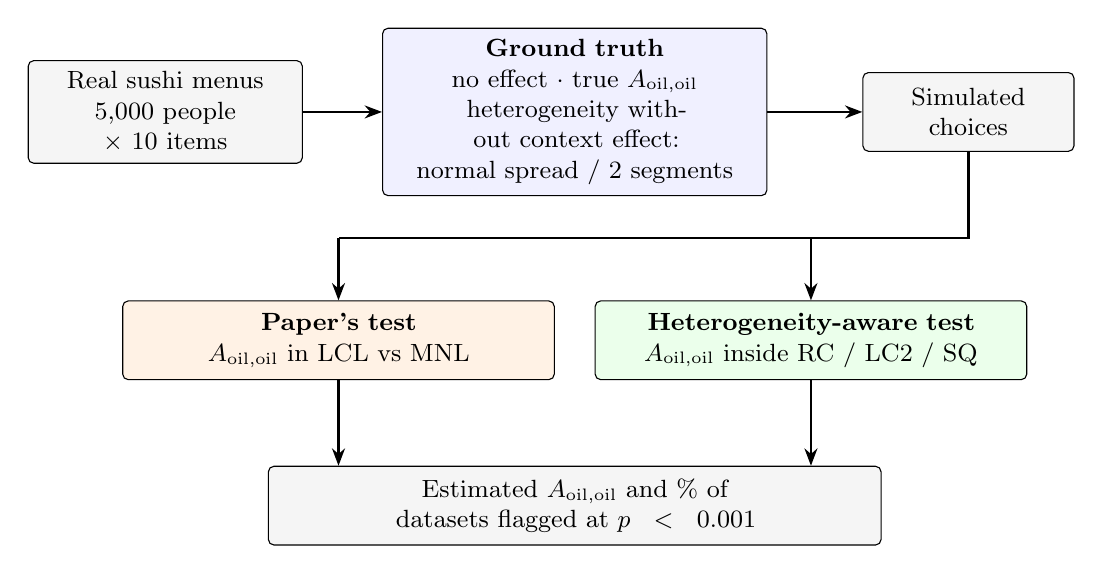
\begin{tikzpicture}[
  box/.style={draw,rounded corners=2pt,align=center,font=\small,inner sep=4pt,minimum height=1.0cm},
  arr/.style={-{Stealth[length=2.2mm]},thick}]
\node[box,fill=gray!8,text width=3.2cm] (menus) at (-5.2,0) {Real sushi menus\\5{,}000 people $\times$ 10 items};
\node[box,fill=blue!6,text width=4.6cm] (truth) at (0,0) {\textbf{Ground truth}\\
  no effect $\cdot$ true $\Aoo$\\heterogeneity without context effect:\\normal spread / 2 segments};
\node[box,fill=gray!8,text width=2.4cm] (sim) at (5.0,0) {Simulated\\choices};
\node[box,fill=orange!10,text width=5.2cm] (paper) at (-3.0,-2.9) {\textbf{Paper's test}\\$\Aoo$ in LCL vs MNL};
\node[box,fill=green!8,text width=5.2cm] (ours) at (3.0,-2.9) {\textbf{Heterogeneity-aware test}\\$\Aoo$ inside RC / LC2 / SQ};
\node[box,fill=gray!8,text width=7.5cm] (out) at (0,-5.0) {Estimated $\Aoo$ and \% of datasets flagged at $p<0.001$};
\draw[arr] (menus) -- (truth);
\draw[arr] (truth) -- (sim);
\draw[thick] (sim.south) -- (5.0,-1.6) -- (-3.0,-1.6);
\draw[arr] (-3.0,-1.6) -- (paper.north);
\draw[arr] (3.0,-1.6) -- (ours.north);
\draw[arr] (paper.south) -- (paper.south |- out.north);
\draw[arr] (ours.south) -- (ours.south |- out.north);
\end{tikzpicture}
\caption{Simulation design. Only the choices are simulated; menus and item features are the real sushi
ones, so the results speak directly to the paper's analysis.}
\label{fig:setup}
\end{figure}

\begin{figure}[!htbp]
\centering
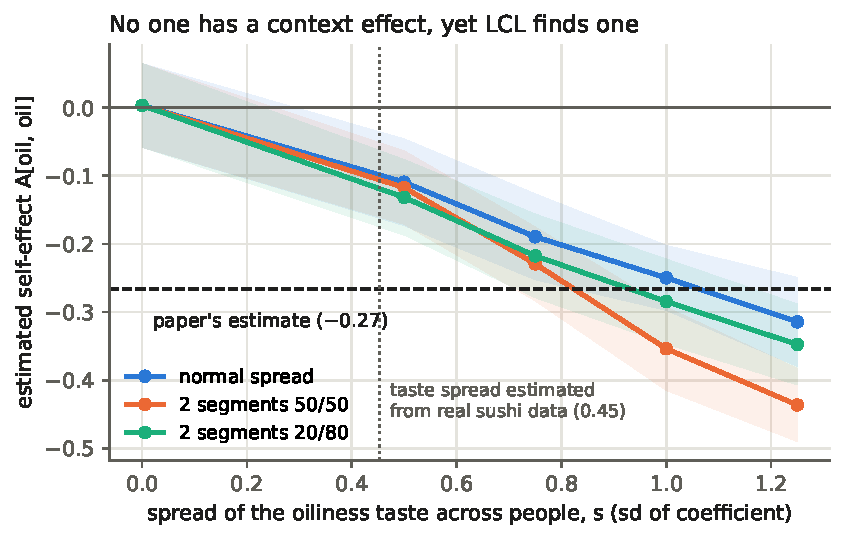
\includegraphics[width=0.78\linewidth]{fig1_spurious_effect.pdf}
\caption{Mean estimate of $\Aoo$ from the paper's one-entry LCL when \emph{no one has a context effect}
but people differ in their oiliness taste (shaded: $\pm1$ sd across replicates). The dotted line marks
the spread we estimate from the real data (\cref{sec:real}).}
\label{fig:spurious}
\end{figure}

\begin{figure}[!htbp]
\centering
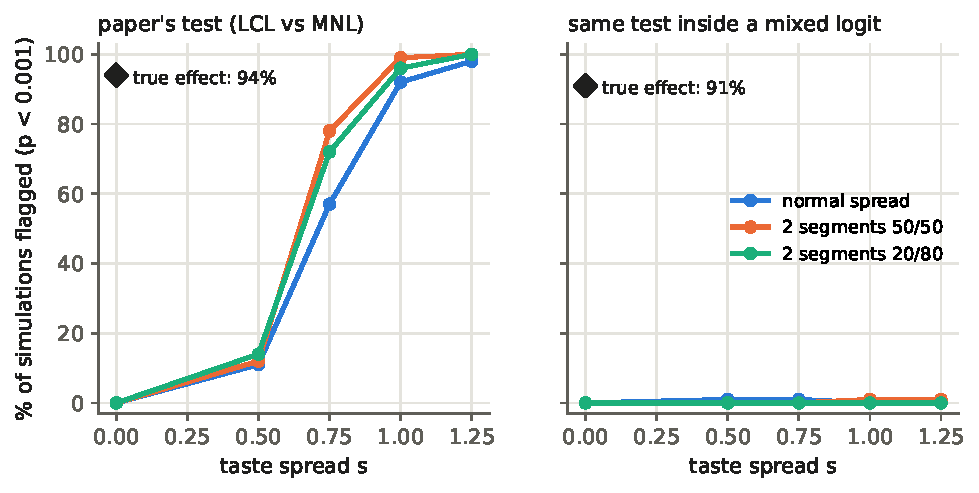
\includegraphics[width=0.92\linewidth]{fig2_rejections.pdf}
\caption{Share of simulated datasets in which $\Aoo$ is significant at $p<0.001$. Left: the paper's test.
Right: the same test inside a normal random-coefficient (mixed) logit. Diamonds: power against a true
effect of the paper's size with no heterogeneity.}
\label{fig:rejections}
\end{figure}

\begin{table}[!htbp]
\centering\small
\setlength{\tabcolsep}{4.5pt}
\begin{tabular}{llcccccccc}
\toprule
 & & \multicolumn{4}{c}{paper's LCL} & \multicolumn{4}{c}{test inside \dots}\\
\cmidrule(lr){3-6}\cmidrule(lr){7-10}
truth & $s$ & mean $\Aoo$ & 36-df & single & $\le$ paper & RC: $\Aoo$ & RC & LC2 & SQ\\
\midrule
no effect & 0 & $+0.00$ & 0\% & 0\% & 0\% & $+0.01$ & 0\% & 0\% & 0\%\\
true effect ($-0.27$) & 0 & $-0.26$ & 21\% & 94\% & 44\% & $-0.25$ & 91\% & 88\% & 91\%\\
effect $-0.15$ + spread & 0.75 & $-0.30$ & 75\% & 98\% & 72\% & $-0.14$ & 10\% & 6\% & 100\%\\
\midrule
\multirow{4}{*}{normal spread} & 0.50 & $-0.11$ & 2\% & 11\% & 1\% & $-0.00$ & 1\% & 0\% & 45\%\\
 & 0.75 & $-0.19$ & 33\% & 57\% & 11\% & $-0.00$ & 1\% & 1\% & 98\%\\
 & 1.00 & $-0.25$ & 88\% & 92\% & 39\% & $+0.02$ & 0\% & 0\% & 100\%\\
 & 1.25 & $-0.31$ & 100\% & 98\% & 77\% & $+0.01$ & 0\% & 0\% & 100\%\\
\midrule
\multirow{4}{*}{2 segments 50/50} & 0.50 & $-0.12$ & 3\% & 12\% & 0\% & $-0.00$ & 0\% & 0\% & 57\%\\
 & 0.75 & $-0.23$ & 61\% & 78\% & 25\% & $-0.02$ & 0\% & 0\% & 100\%\\
 & 1.00 & $-0.35$ & 100\% & 99\% & 94\% & $-0.08$ & 1\% & 0\% & 100\%\\
 & 1.25 & $-0.44$ & 100\% & 100\% & 100\% & $-0.11$ & 1\% & 0\% & 100\%\\
\midrule
\multirow{4}{*}{2 segments 20/80} & 0.50 & $-0.13$ & 4\% & 14\% & 2\% & $-0.01$ & 0\% & 0\% & 76\%\\
 & 0.75 & $-0.22$ & 60\% & 72\% & 26\% & $+0.00$ & 0\% & 0\% & 100\%\\
 & 1.00 & $-0.28$ & 99\% & 96\% & 60\% & $+0.04$ & 0\% & 0\% & 100\%\\
 & 1.25 & $-0.35$ & 100\% & 100\% & 93\% & $+0.05$ & 0\% & 0\% & 100\%\\
\bottomrule
\end{tabular}
\caption{Simulation results (100 replicates per row; rates are $\pm5$--10 points). ``36-df'' and ``single'':
the paper's whole-model and one-entry tests. ``$\le$ paper'': significant \emph{and} at least as negative
as $-0.266$. Right block: the single-entry test inside a normal random coefficient (RC), two latent
classes (LC2) or a squared term (SQ) on oiliness.}
\label{tab:sim}
\end{table}

\paragraph{Results.}
\Cref{fig:spurious,fig:rejections} and \cref{tab:sim} show four things.
\begin{enumerate}
\item \textbf{Heterogeneity alone reproduces the finding.} With no context effect anywhere, a taste spread
      of $s\approx0.8$--$1.0$ standard deviations gives the paper's $-0.27$ on average, and the paper's single
      test flags an effect in 57--99\% of datasets. Both types of heterogeneity do this; segments produce a
      larger effect than a normal spread of the same variance, consistent with third-order terms.
\item \textbf{Testing inside a mixed logit fixes the size and keeps the power.} The same LRT inside RC or LC2
      rejects in 0--1\% of heterogeneity datasets at every $s$, yet still detects the true effect 91\% (RC)
      and 88\% (LC2) of the time, against 94\% for the paper's test. When both a context effect and
      heterogeneity are present, RC recovers $\Aoo=-0.14$ for a true $-0.15$; the paper's test reports
      $-0.30$. (Power is low at this smaller effect size.) A normal RC fitted to segment data leaves a small
      residual at large $s$ but rarely a significant one.
\item \textbf{A squared term is not a fix.} Inside SQ the false-positive rate is \emph{higher} (45--100\%),
      as \cref{prop:expansion} predicts.
\item \textbf{A cheap diagnostic.} At equal parameter counts (MNL + one $A$ entry vs MNL + one variance), the
      mixed logit fits better in 100\% of heterogeneity datasets and 0\% of true-effect datasets.
\end{enumerate}

%======================================================================
\section{Real sushi data}
\label{sec:real}

\subsection{Is there taste heterogeneity, and does the effect survive it?}

\Cref{tab:real} fits heterogeneity-aware models to the paper's data (one choice per person) and tests
$\Aoo$ inside each one.

\begin{table}[!htbp]
\centering\small
\begin{tabular}{lcccl}
\toprule
base model & log-lik. & $\Aoo$ & LRT ($p$) & heterogeneity estimate\\
\midrule
MNL (the paper's test) & $-9821.4$ & $-0.266$ & 23.1 ($1.6\times10^{-6}$) & ---\\
+ squared oiliness & $-9820.7$ & $-0.296$ & 27.5 ($1.5\times10^{-7}$) & curvature $0.02$\\
RC on oiliness & $-9807.5$ & $-0.214$ & 10.9 ($9.4\times10^{-4}$) & sd $0.45$\\
RC on all features & $-9804.3$ & $-0.220$ & 10.7 ($1.0\times10^{-3}$) & sd: oil $0.47$, price $0.31$, rest $\approx0$\\
2 classes on oiliness & $-9807.1$ & $-0.214$ & 10.9 ($9.6\times10^{-4}$) & 48\% / 52\%\\
2 classes on all features & $-9799.0$ & $-0.207$ & 9.8 ($1.7\times10^{-3}$) & \\
demographics & $-9757.5$ & $-0.265$ & 22.7 ($1.9\times10^{-6}$) & gender, age, east/west\\
demographics + RC all & $-9741.0$ & $-0.216$ & 10.4 ($1.2\times10^{-3}$) & \\
\bottomrule
\end{tabular}
\caption{Real sushi data, one choice per person. The log-likelihood is that of the base model; the LRT
tests adding $\Aoo$ to it.}
\label{tab:real}
\end{table}

\begin{itemize}
\item \textbf{Heterogeneity is present.} Letting the oiliness taste vary (one extra parameter) improves the
      log-likelihood by 13.9 over MNL and beats the paper's one-entry LCL ($-9809.8$) at the same number of
      parameters: heterogeneity is the better single explanation of the data.
\item \textbf{The effect shrinks but survives marginally.} Inside every heterogeneity model, $\Aoo$ falls to
      about $-0.21$ and its $p$-value rises about 600-fold, to the paper's own threshold of $10^{-3}$.
\item \textbf{Observed demographics do not explain it.} Gender, age and region shift tastes (women prefer
      lighter sushi) but leave $\Aoo$ unchanged.
\item \textbf{Other effects weaken too.} Inside RC on all features, price-on-price goes from $p=4\times10^{-4}$ to
      $0.014$ and price-on-oiliness from $6\times10^{-4}$ to $0.039$. The 36-entry whole-model test, however,
      remains significant (LRT $97\to78$, $p=7\times10^{-5}$).
\end{itemize}

\subsection{How much of the effect can the observed heterogeneity produce?}

We fitted heterogeneity models \emph{without} context effects to the sushi data, re-simulated 200
datasets from each on the real menus, and reran the paper's analysis (\cref{fig:boot}). Taste spreads of
the size the data show produce $\Aoo\approx-0.09$ on average --- about a third of the observed $-0.27$ ---
and significant at $p<0.001$ in 3--6\% of datasets (12\% for a three-class model), but an estimate as
extreme as $-0.266$ almost never ($\le0.5\%$) and never the paper's whole-model LRT of 97. With only one
choice per person, then, heterogeneity explains part of the effect but not all of it.

\begin{figure}[!htbp]
\centering
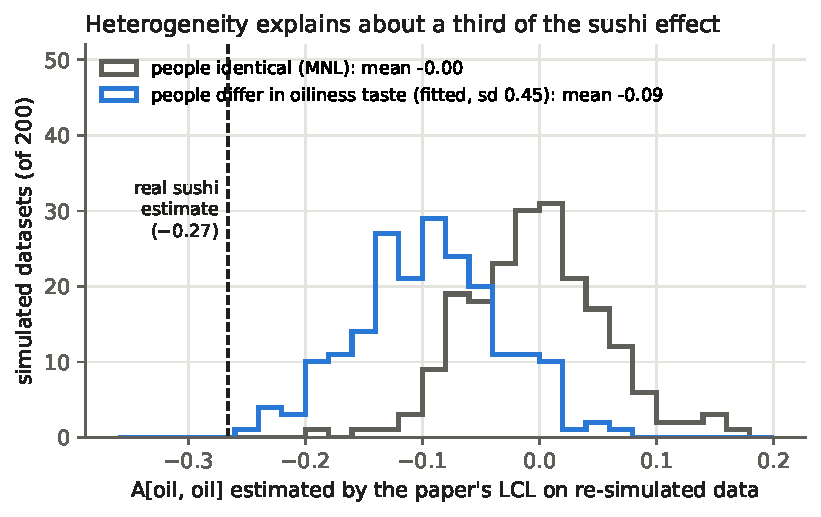
\includegraphics[width=0.75\linewidth]{fig3_bootstrap.pdf}
\caption{Parametric bootstrap: the paper's $\Aoo$ estimated on 200 datasets re-simulated from an MNL and from a
random-coefficient model fitted to sushi (neither has a context effect). Two-class and all-feature
heterogeneity models give nearly identical histograms (means $-0.09$).}
\label{fig:boot}
\end{figure}

\subsection{Using the full rankings to identify individual tastes}

With one choice per person, a person's taste and the menu's context are hard to separate. But every
respondent ranked all ten items, and the paper keeps only the top one. Reading a ranking as successive
choices (best of 10, then best of the remaining 9, \dots; the rank-ordered logit~\cite{beggs81}) gives
$k$ choices per person. Each person's taste $\eta_n$ is shared across their $k$ choices while the menu
mean changes from stage to stage, which is exactly the variation needed to separate heterogeneity from
context. We fitted panel RC models on all six features, with and without $\Aoo$.

\begin{table}[!htbp]
\centering\small
\begin{tabular}{ccc}
\toprule
choices per person $k$ & LCL, no heterogeneity: $\Aoo$ ($p$) & panel RC + $\Aoo$: $\Aoo$ ($p$)\\
\midrule
1 & $-0.266$ ($1.6\times10^{-6}$) & $-0.220$ ($1.0\times10^{-3}$)\\
2 & $-0.243$ ($1.6\times10^{-10}$) & $\mathbf{-0.064}$ ($\mathbf{0.23}$)\\
3 & $-0.228$ ($5.7\times10^{-14}$) & $\mathbf{+0.015}$ ($\mathbf{0.73}$)\\
\bottomrule
\end{tabular}
\caption{Real sushi data using each respondent's top-$k$ ranked choices.}
\label{tab:panel}
\end{table}

\Cref{tab:panel} shows that once two or three choices per person are used, the effect disappears inside the
panel RC model, while an LCL that ignores heterogeneity becomes \emph{more} significant.

\paragraph{Is the panel test trustworthy?}
A vanishing estimate is only informative if the test could have detected the effect. We simulated 50
ranking datasets per truth on the real menus, stage by stage (so that a true LCL effect acts on the
remaining items at every stage), with tastes taken from the sushi panel fit (\cref{tab:panelcheck}).

\begin{table}[!htbp]
\centering\small
\begin{tabular}{lccccc}
\toprule
 & & \multicolumn{2}{c}{LCL, no heterogeneity} & \multicolumn{2}{c}{panel RC + $\Aoo$}\\
\cmidrule(lr){3-4}\cmidrule(lr){5-6}
truth & $k$ & mean $\Aoo$ & flagged & mean $\Aoo$ & flagged\\
\midrule
people differ, no context effect & 2 & $-0.16$ & 78\% & $+0.00$ & 0\%\\
 & 3 & $-0.22$ & 100\% & $+0.01$ & 0\%\\
people differ + $\Aoo=-0.266$ & 2 & $-0.38$ & 100\% & $-0.25$ & 94\%\\
 & 3 & $-0.43$ & 100\% & $-0.26$ & 100\%\\
no heterogeneity, $\Aoo=-0.266$ & 2 & $-0.26$ & 100\% & $-0.26$ & 100\%\\
 & 3 & $-0.27$ & 100\% & $-0.26$ & 100\%\\
\bottomrule
\end{tabular}
\caption{Validation of the ranking-based test (50 simulated datasets per row; flagged = $p<0.001$).}
\label{tab:panelcheck}
\end{table}

The panel test has the right size (0\% false positives) and 94--100\% power against an effect of the
paper's size, so the real-data estimates of $-0.06$ and $+0.02$ are strong evidence against such an
effect. The LCL that ignores heterogeneity is badly biased on ranking data: later menus depend on the
person's own earlier picks, so taste heterogeneity becomes choice-set confounding~\cite{tub21}. This
explains why its estimate grows more significant as $k$ increases in \cref{tab:panel}.

\subsection{First pick versus later picks}

Finally, we allowed separate self-effects for the first pick (from the full menu) and for later picks,
in the panel model with $k=2$ and $k=3$. Without heterogeneity, both stages show the same effect
($\approx-0.23$ and $-0.25$, all $p<10^{-4}$), as a pure heterogeneity artefact would. With heterogeneity
modelled, later picks show nothing ($+0.04$, $p=0.61$; $+0.09$, $p=0.06$), but a \emph{first-pick} effect
of $-0.16$ ($p=0.017$) and $-0.14$ ($p=0.034$) remains. This could be a genuine reaction to the first
look at a menu, or heterogeneity our diagonal normal model does not capture (for example correlated
tastes); our data cannot separate the two. Either way, it is about half the paper's estimate and far from
$p=10^{-6}$.

%======================================================================
\section{Discussion}
\label{sec:discussion}

\paragraph{What we learned.}
\begin{enumerate}
\item \textbf{LCL self-effects are confounded with taste heterogeneity.} In theory
      (\cref{prop:expansion}) and in simulation, context-free choosers who differ in taste produce
      significant negative self-effects --- the similarity-effect signature the paper interprets. This is
      the classic point that the similarity effect can be explained by heterogeneity
      instead~\cite{tversky72,mcfadden00} and that aggregation can create context
      effects~\cite{hkl00,lhl16}, made precise for LCL. Randomising menus does not protect against it.
\item \textbf{On sushi, the headline effect does not survive.} Heterogeneity is clearly present. With one
      choice per person, it accounts for about a third of the effect and leaves the rest borderline. With
      the rankings that identify individual tastes, a validated test finds nothing at later picks and only a
      weak first-pick effect. The paper's causal reading is not supported.
\item \textbf{The fix is cheap and keeps what is good about LCL.} Test context effects \emph{inside} a
      mixed logit or latent-class model, and use repeated choices per person where they exist. Each fit
      takes seconds, the test has the right size, and it loses little power. Adding flexible functional
      form (a squared term) is not a substitute.
\end{enumerate}

\paragraph{Which context effects can heterogeneity mimic?}
Any mixture of logits --- normal, latent-class or otherwise --- is a random utility model, and every random
utility model satisfies \emph{regularity}: adding an item to a menu can never raise the probability of
choosing an item already on it~\cite{bm60}. Taste heterogeneity can therefore produce similarity-type
patterns such as negative self-effects, but never an effect that violates regularity, such as the
attraction (decoy) effect~\cite{hpp82}. This gives a sharp scope for our critique. It applies to LCL entries
whose implied choice probabilities stay consistent with regularity, which includes the oiliness self-effect.
Effects that imply regularity violations cannot be explained by heterogeneity alone; positive self-effects
such as the paper's car-alt ``truck on truck'' need another explanation, for example the choice-set
tailoring the authors themselves uncovered. Checking whether a fitted $A$ implies any regularity
violations on the observed menus would be a simple screening test for which effects need a
heterogeneity-aware test.

\paragraph{What we do not claim.}
We do not claim that LCL detects nothing: the whole-model sushi test remains significant after allowing
for heterogeneity, so some context structure may be real, and we have not re-examined the paper's other
datasets. Our claim is specific to self-effects of the similarity type and to the oiliness result.

\paragraph{Limitations.}
\begin{itemize}
\item The rank-ordered model assumes the same utility at every rank. Deeper ranks are known to be answered
      less carefully, with more noise~\cite{hr87}: at $k=5$ the panel estimate becomes $+0.12$
      ($p=9\times10^{-4}$), so we stop at $k=3$ and validate only $k\le3$ by simulation.
\item Our heterogeneity models are diagonal normal and up to three classes; correlated tastes were not
      tried.
\item Simulation rates are based on 100 replicates (50 for the panel check), so they carry
      $\pm5$--10 percentage points of noise.
\item \Cref{prop:expansion} is a small-$s$ result; for $s\gtrsim0.5$ it is qualitative only.
\item How strongly heterogeneity leaks into $A$ depends on the menu design: in a pilot with Gaussian
      synthetic items, the same spread produced a much smaller self-effect ($\approx-0.06$ at $s=1$) than
      on the real sushi menus.
\end{itemize}

\paragraph{Next steps.}
Apply the same heterogeneity-aware tests to the paper's other datasets (expedia, car-alt, and the network
datasets); characterise the third-order term that separates normal from segmented heterogeneity; and test
whether the remaining first-pick effect survives richer (correlated) heterogeneity models.

%======================================================================
\begin{thebibliography}{99}\small
\bibitem{tb21} K.~Tomlinson and A.~R.~Benson. Learning interpretable feature context effects in discrete
  choice. In \emph{Proc.\ KDD}, 2021.
\bibitem{kamishima03} T.~Kamishima. Nantonac collaborative filtering: recommendation based on order
  responses. In \emph{Proc.\ KDD}, pp.~583--588, 2003.
\bibitem{tub21} K.~Tomlinson, J.~Ugander and A.~R.~Benson. Choice set confounding in discrete choice. In
  \emph{Proc.\ KDD}, 2021.
\bibitem{mcfadden00} D.~McFadden and K.~Train. Mixed MNL models for discrete response. \emph{Journal of
  Applied Econometrics}, 15(5):447--470, 2000.
\bibitem{train09} K.~Train. \emph{Discrete Choice Methods with Simulation}, 2nd ed. Cambridge University
  Press, 2009.
\bibitem{tversky72} A.~Tversky. Elimination by aspects: a theory of choice. \emph{Psychological Review},
  79(4):281--299, 1972.
\bibitem{beggs81} S.~Beggs, S.~Cardell and J.~Hausman. Assessing the potential demand for electric cars.
  \emph{Journal of Econometrics}, 17(1):1--19, 1981.
\bibitem{hkl00} J.~W.~Hutchinson, W.~A.~Kamakura and J.~G.~Lynch. Unobserved heterogeneity as an
  alternative explanation for ``reversal'' effects in behavioral research. \emph{Journal of Consumer
  Research}, 27(3):324--344, 2000.
\bibitem{lhl16} S.~X.~Liew, P.~D.~L.~Howe and D.~R.~Little. The appropriacy of averaging in the study of
  context effects. \emph{Psychonomic Bulletin \& Review}, 23(5):1639--1646, 2016.
\bibitem{heckman81} J.~J.~Heckman. Heterogeneity and state dependence. In S.~Rosen (ed.), \emph{Studies in
  Labor Markets}, pp.~91--140. University of Chicago Press, 1981.
\bibitem{rvb11} R.~P.~Rooderkerk, H.~J.~van Heerde and T.~H.~A.~Bijmolt. Incorporating context effects into
  a choice model. \emph{Journal of Marketing Research}, 48(4):767--780, 2011.
\bibitem{spu19} A.~Seshadri, A.~Peysakhovich and J.~Ugander. Discovering context effects from raw choice
  data. In \emph{Proc.\ ICML}, 2019.
\bibitem{su20} A.~Seshadri and J.~Ugander. Fundamental limits of testing the independence of irrelevant
  alternatives in discrete choice. arXiv:2001.07042, 2020.
\bibitem{hr87} J.~A.~Hausman and P.~A.~Ruud. Specifying and testing econometric models for rank-ordered
  data. \emph{Journal of Econometrics}, 34(1--2):83--104, 1987.
\bibitem{bm60} H.~D.~Block and J.~Marschak. Random orderings and stochastic theories of responses. In
  I.~Olkin et al.\ (eds.), \emph{Contributions to Probability and Statistics}, pp.~97--132. Stanford
  University Press, 1960.
\bibitem{hpp82} J.~Huber, J.~W.~Payne and C.~Puto. Adding asymmetrically dominated alternatives: violations
  of regularity and the similarity hypothesis. \emph{Journal of Consumer Research}, 9(1):90--98, 1982.
\end{thebibliography}

%======================================================================
\appendix
\section{Implementation details}
\label{app:impl}

\begin{itemize}
\item \textbf{Code.} All models are one PyTorch class: utility $(\theta+A\xb_C+Bw_n+\eta_n)^\top x_i +
      \sum_kq_kx_{ik}^2$, with any subset of $A$ free, optional demographics $w_n$, and $\eta_n$ either normal
      (simulated with 200 scrambled Sobol draws per person, randomly shifted; 100 in panel models) or latent
      classes. When a person has several choices, $\eta_n$ is shared across them.
\item \textbf{Estimation.} Exact maximum likelihood with L-BFGS (strong Wolfe line search) in double
      precision and no regularisation, so LRTs are clean. Non-convex models use several random restarts.
      Nested models are fitted from each other's optimum, which guarantees non-negative LRT statistics.
\item \textbf{Tests.} We only use LRTs for entries of $A$, which are regular one-degree-of-freedom tests.
      Variance parameters lie on a boundary~\cite{train09}, and we do not test them with LRTs.
\item \textbf{Run time.} Reproduction and the theory check take about a minute; the simulation study takes
      about 4 hours on 8 CPU cores, and the bootstrap and ranking checks take about an hour together.
\item \textbf{Data.} The sushi data cannot be redistributed; the code downloads it from the author's site.
\end{itemize}

\end{document}
